\begin{appendix}
\chapter{Evaluation results}
This section will give an overview of the raw results gathered by the evaluations performed on the different prototypes.
\section{Capacitive chair posture recognition}
\label{ch:app_capchair_eval}
This section provides raw data of the first posture recognition test performed using the capacitive chair. 
\subsection{Evaluation setup}
Short study with 10 participants. Three poses and a non-pose:
\begin{itemize}
\item Sitting upright
\item Sitting hunched
\item Slouching on chair
\item Close to chair - disturber
\end{itemize}

The persons were given a short introduction, the different postures were displayed, and finally the persons were asked to perform the postures in order. When testing “close-to-chair” the subjects were asked to rattle at the chair, stand close, move it around and thus disturb the potential sensor readings. Each class was tested for 10 seconds, collecting 200 samples. 

\subsection{Raw results}
\begin{table}[htbp]
  \centering
  \caption{Percentage of correctly classified postures using manually set classifier}
    \begin{tabularx}{\linewidth}{XXXXXXXXXXXX}
    \toprule
          & S1    & S2    & S3    & S4    & S5    & S6    & S7    & S8    & S9    & S10   & Avg \\
    \midrule
    Upright & 100   & 100   & 100   & 100   & 100   & 100   & 100   & 100   & 100   & 100   & 100 \\
    Hunched & 100   & 100   & 100   & 100   & 86    & 100   & 100   & 100   & 100   & 100   & 98,6 \\
    Slouch & 100   & 100   & 100   & 100   & 100   & 100   & 100   & 100   & 55    & 100   & 95,5 \\
    Disturber & 100   & 100   & 100   & 100   & 100   & 100   & 100   & 100   & 100   & 100   & 100 \\
    \bottomrule
    \end{tabularx}%
  \label{tab:app_eval_chair_raw1}%
\end{table}%
\subsection{Postures}
\begin{minipage}{\linewidth}
\centering
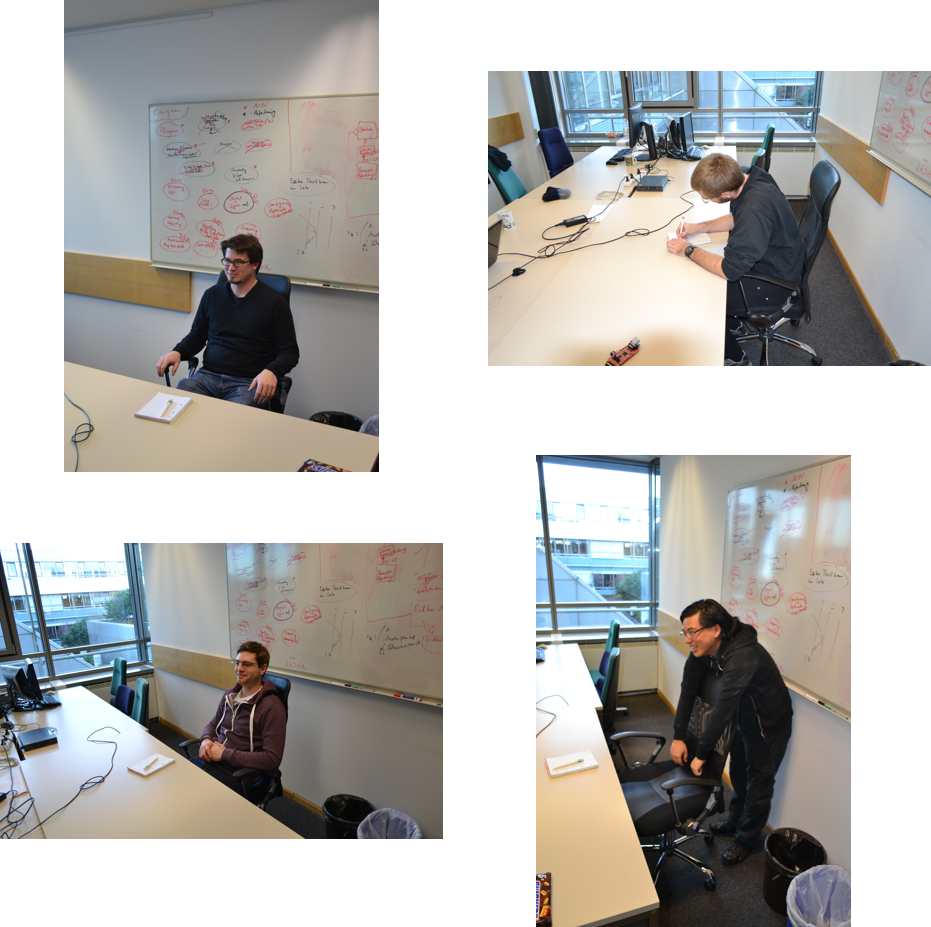
\includegraphics[width=0.8\textwidth]{images/app_eval_chair1}
\captionof{figure}{\emph{Top left} upright posture. \emph{Top right} hunched posture. \emph{Bottom left} slouched posture. \emph{Bottom right} disturber posture}
\label{fig:disc_unob_elec}
\end{minipage}

\section{Capacitive Chair - working situation recognition}
\begin{minipage}{\linewidth}
\centering
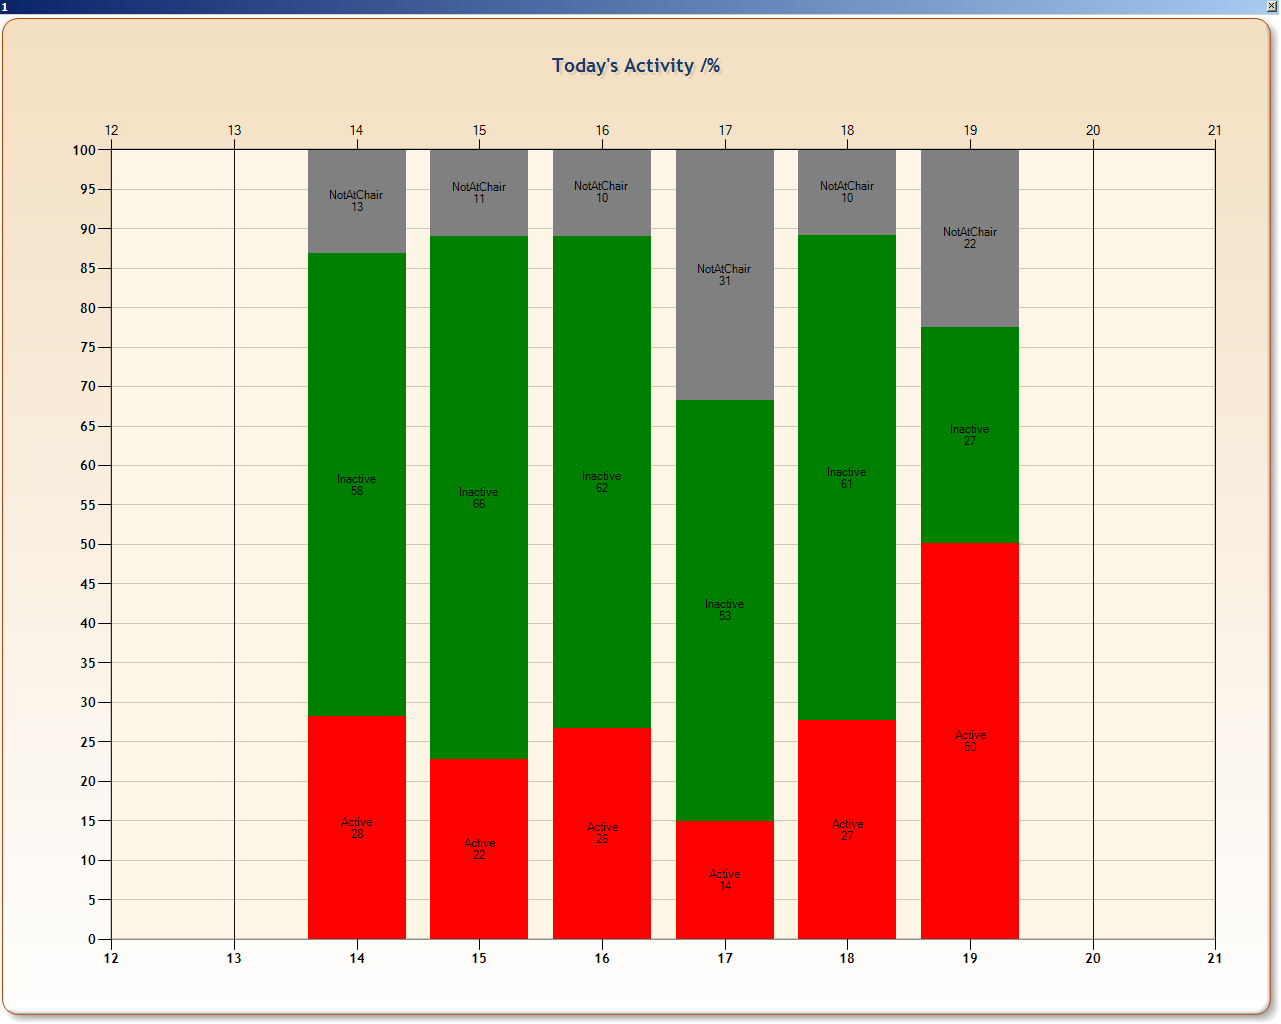
\includegraphics[width=0.6\textwidth]{images/workact_day1}
\captionof{figure}{Work activity day 1}
\label{fig:workact_day1}
\end{minipage}

\begin{minipage}{\linewidth}
\centering
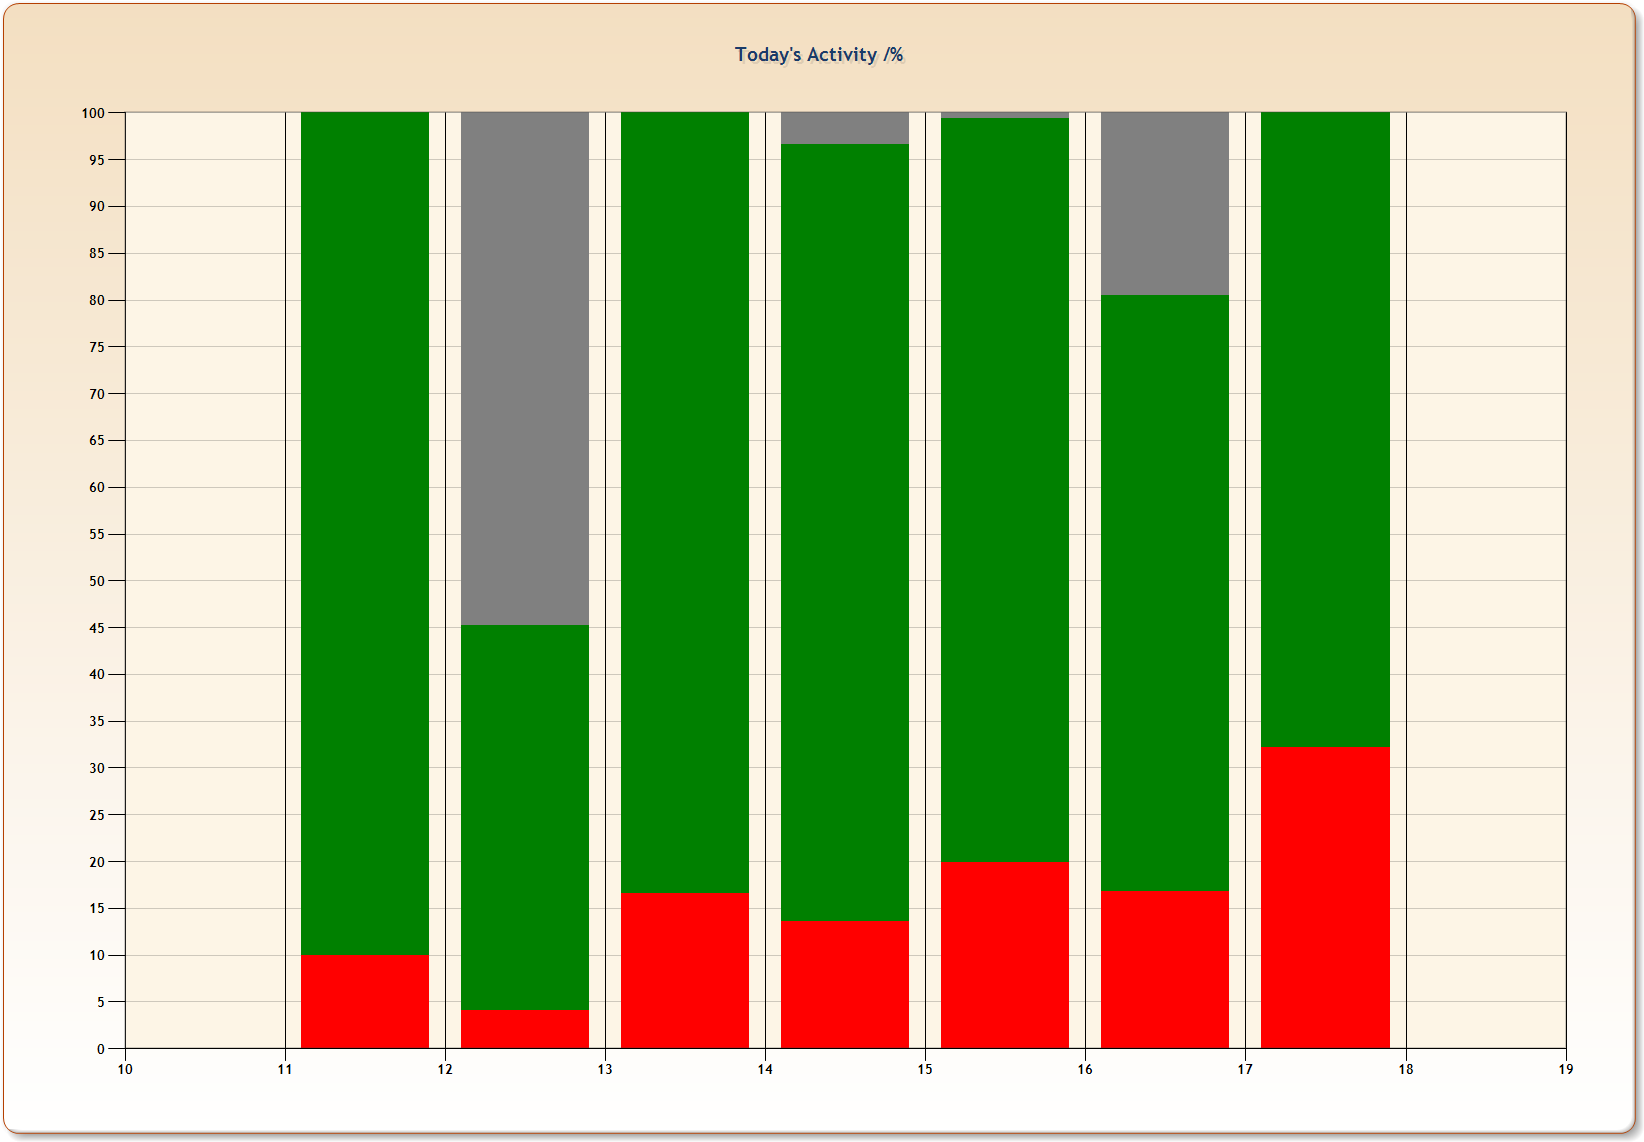
\includegraphics[width=0.6\textwidth]{images/workact_day2}
\captionof{figure}{Work activity day 2}
\label{fig:workact_day2}
\end{minipage}

\begin{minipage}{\linewidth}
\centering
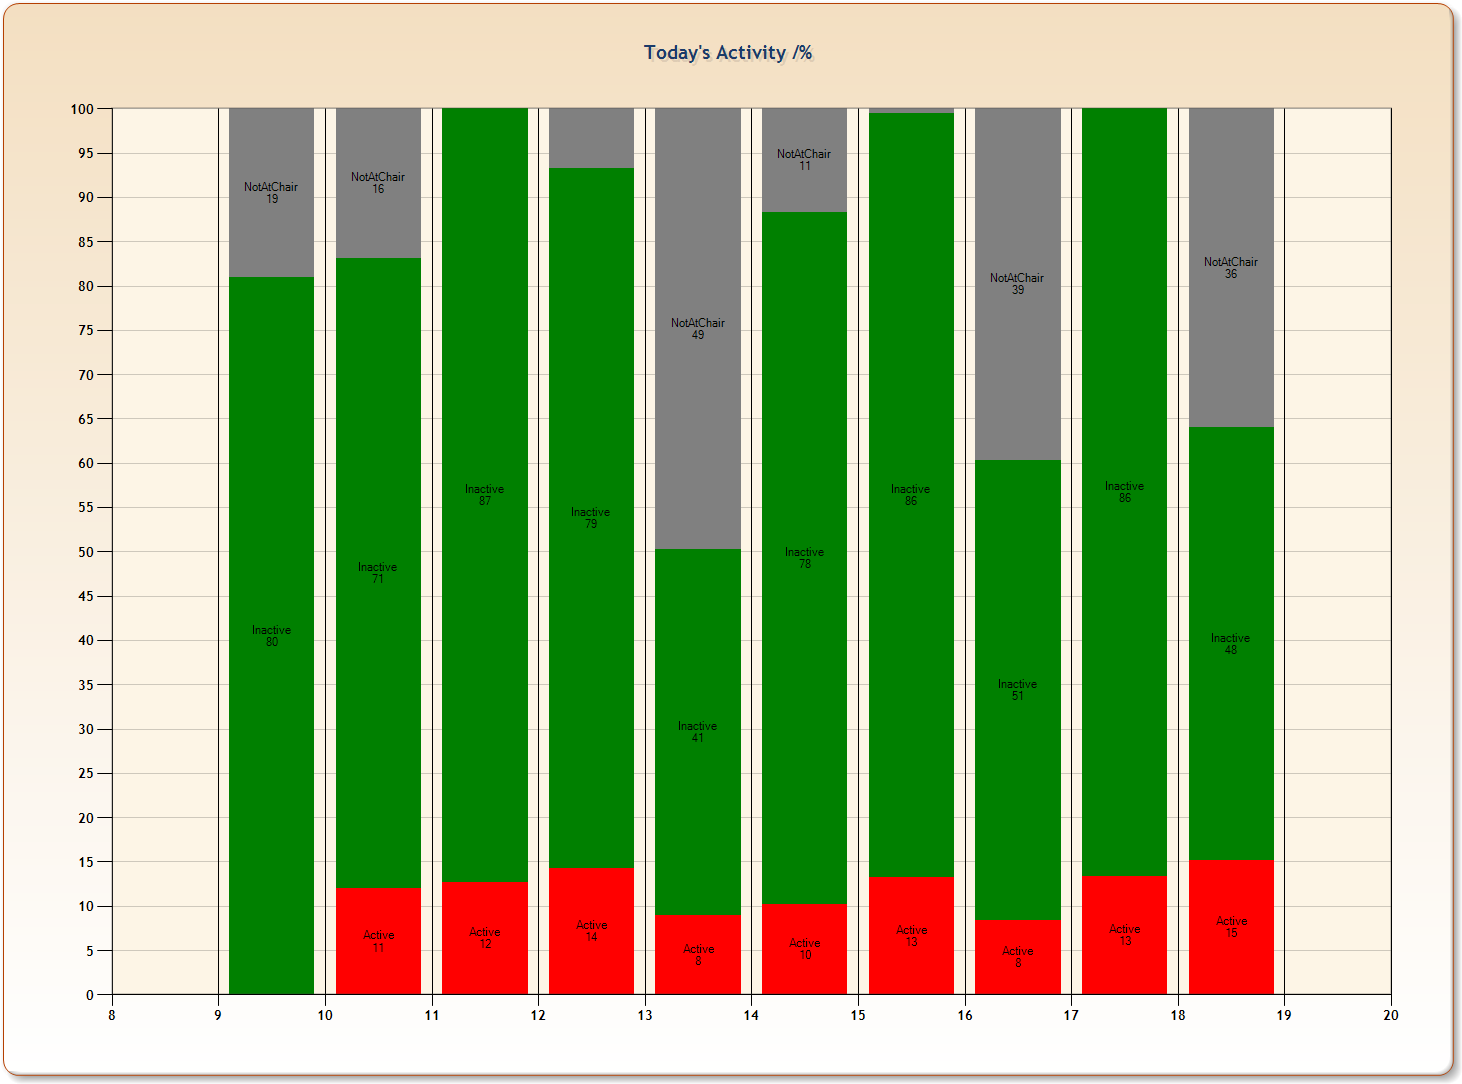
\includegraphics[width=0.6\textwidth]{images/workact_day3}
\captionof{figure}{Work activity day 3}
\label{fig:workact_day3}
\end{minipage}


\section{CapTap evaluation}
\subsection{Questionnaire}
\begin{itemize}
\item G1 Experience with touch screen systems (none = 1, daily usage = 10)
\item G2 Experience with gesture recognition systems (none = 1, daily usage = 10)
\item Q1 Do you agree that the required tasks were easy and precise to perform? (Not agree = 1, Strong agree = 10)
\item Q2 Was the CapTap to be intuitive in its usage? (Not agree = 1, Strong agree = 10)
\item Q3 I could control the different layers in the painter application? (Not agree = 1, Strong agree = 10)
\item Q4 I could control the different interactions in the test run? (Not agree = 1, Strong agree = 10)
\item Q5 Do you prefer finger swipes or hand swipes?
(Finger swipe = 1, Hand swipe = 10)
\item Q6Do you prefer finger taps or knuckle knocks? (Finger taps = 1, Knuckle knocks = 10)
\item Q7 The CapTap should support more than three interaction layers? (Not agree = 1, Strong agree = 10)
\item Q8 Do you agree that CapTap is an interesting form of interaction device? (Not agree = 1, Strong agree = 10)
\item Q9 Would you consider using an input device like CapTap for a longer period of time? (Not at all = 1, I would like to use it = 10)
\item Q10 What did you particularly like about the CapTap?
\item Q11 What did you particularly dislike about the CapTap?
\end{itemize}

\subsection{Raw results}
The table denotes the results of the different touch points as explained in the descriptive section. The T's refer to the times of the three different interaction speed runs.

\begin{landscape}
\begin{table}[htbp]
  \footnotesize
  \centering
  \caption{CapTap evaluation raw results}
    \begin{tabular}{rrrrrrrrrrrrrrrrrrrrrrrrr}
    \toprule
    Subject & 1     & 1D    & 2     & 2D    & 3     & 3D    & 4     & 4D    & 5     & 5D    & 6     & 6D    & 7     & 8     & 9     & 10    & 11    & 12    & 13    & 14    & 15    & T1    & T2    & T3 \\
    \midrule
    S1    & 3     & 3     & 3     & 3     & 3     & 3     & 1     & 3     & 2     & 0     & 1     & 2     & 3     & 3     & 3     & 3     & 3     & 3     & 3     & 3     & 3     & 45,38 & 41,57 & 33,94 \\
    S2    & 3     & 3     & 3     & 3     & 3     & 3     & 3     & 3     & 3     & 3     & 3     & 3     & 3     & 3     & 3     & 3     & 3     & 3     & 3     & 3     & 3     & 43,12 & 41,83 & 36,94 \\
    S3    & 3     & 2     & 3     & 3     & 3     & 3     & 3     & 2     & 2     & 2     & 2     & 2     & 2     & 3     & 0     & 3     & 3     & 3     & 1     & 3     & 3     & 51,38 & 34,42 & 31,33 \\
    S4    & 3     & 3     & 3     & 3     & 3     & 3     & 3     & 3     & 3     & 3     & 3     & 3     & 3     & 3     & 3     & 3     & 3     & 3     & 3     & 3     & 3     & 27,28 & 34,17 & 24,29 \\
    S5    & 3     & 2     & 2     & 3     & 3     & 3     & 3     & 1     & 3     & 3     & 3     & 1     & 2     & 3     & 3     & 3     & 3     & 3     & 2     & 3     & 2     & 34,66 & 48,11 & 45,35 \\
    S6    & 3     & 3     & 3     & 3     & 3     & 3     & 3     & 3     & 3     & 2     & 2     & 1     & 3     & 3     & 3     & 3     & 3     & 3     & 1     & 3     & 1     & 39,28 & 42,62 & 47,72 \\
    S7    & 3     & 3     & 3     & 3     & 3     & 3     & 3     & 3     & 3     & 2     & 3     & 3     & 0     & 1     & 3     & 1     & 3     & 3     & 1     & 3     & 1     & 40,87 & 33,56 & 25,95 \\
    S8    & 3     & 3     & 3     & 3     & 3     & 3     & 2     & 0     & 1     & 1     & 3     & 0     & 3     & 3     & 3     & 3     & 3     & 3     & 3     & 3     & 1     & 47,14 & 37,43 & 32,72 \\
    S9    & 3     & 3     & 3     & 3     & 3     & 2     & 2     & 3     & 1     & 0     & 2     & 2     & 0     & 3     & 0     & 3     & 3     & 3     & 1     & 3     & 2     & 39,71 & 33,78 & 26,63 \\
    S10   & 3     & 3     & 3     & 3     & 3     & 3     & 2     & 0     & 3     & 0     & 2     & 0     & 3     & 3     & 1     & 3     & 3     & 3     & 2     & 1     & 1     & 32,35 & 32,2  & 29,31 \\
    Ergebnis & 30    & 28    & 29    & 30    & 30    & 29    & 25    & 21    & 24    & 16    & 24    & 17    & 22    & 28    & 22    & 28    & 30    & 30    & 20    & 28    & 20    & 40,117 & 37,969 & 33,418 \\
    \bottomrule
    \end{tabular}%
  \label{tab:app_eval_captap_raw_quant}%
\end{table}%
\end{landscape}
\begin{landscape}
% Table generated by Excel2LaTeX from sheet 'Tabelle3'
\begin{table}[htbp]
  \footnotesize
  \centering
  \caption{CapTap questionnaire results}
    \begin{tabular}{rrrrrrrrrrrrm{4.5cm}m{4.5cm}}
    \toprule
    Subject & G1    & G2    & Q1    & Q2    & Q3    & Q4    & Q5    & Q6    & Q7    & Q8    & Q9    & Q10   & Q11 \\
    \midrule
    S1    & 10    & 5     & 6     & 9     & 9     & 8     & 8     & 1     & 6     & 10    & 9     & unsichtbare Sensorik im vertrauten Möbelstück, Gesten über Tisch & Präzision nicht gut genug \\
    S2    & 10    & 9     & 6     & 8     & 6     & 8     & 7     & 3     & 3     & 7     & 6     & Nice idea of embedding interaction into everyday furniture & area is too large, interaction is exhausting, demonstrator table not suitable \\
    S3    & 10    & 4     & 10    & 10    & 5     & 10    & 10    & 1     & 1     & 10    & 7     & tactility, intuitive and invisible & some areas hard to reach when sitting in front \\
    S4    & 10    & 8     & 8     & 9     & 8     & 9     & 2     & 1     & 4     & 10    & 8     &       & some errors in interaction \\
    S5    & 10    & 3     & 10    & 8     & 8     & 8     & 2     & 1     & 6     & 9     & 8     & touchpad like control on table & knocking, interaction disturbed by knee \\
    S6    & 10    & 8     & 8     & 9     & 7     & 8     & 3     & 3     & 3     & 9     & 8     & unobtrusive integration in furniture, intuitive interaction & delay in recognition \\
    S7    & 10    & 10    & 10    & 10    & 5     & 10    & 3     & 2     & 5     & 10    & 8     & Eingaben mit und ohne Kontakt, Auswahl über Tap intuitiv, Schnelle Eingewöhnung in Layer mit Farben & Beine werden erkannt, große Interaktionsarea, Verzerrungen im Zeichenprogramm \\
    S8    & 10    & 3     & 7     & 8     & 7     & 9     & 2     & 2     & 1     & 7     & 4     & ease of use, low learning curve, big variety of input modalities & interaction less precise in some areas \\
    S9    & 10    & 3     & 8     & 9     & 4     & 7     & 7     & 10    & 3     & 9     & 3     & knockin on heaven's door & tap didn't work - required more than one tap to recognize \\
    S10   & 4     & 7     & 8     & 9     & 7     & 9     & 2     & 2     & 7     & 10    & 8     & different interaction possibilities & detection of knees, difficulty to stay in layer \\
    Ergebnis & 9,4   & 6     & 8,1   & 8,9   & 6,6   & 8,6   & 4,6   & 2,6   & 3,9   & 9,1   & 6,9   &       &  \\
    \bottomrule
    \end{tabular}%
  \label{tab:app_eval_captap_raw_quest}%
\end{table}%
\end{landscape}

\section{Active Armrest evaluation results}
\subsection{Questionnaire}
\begin{itemize}
\item G1 Experience with touch screen systems (none = 1, daily usage = 10)
\item G2 Experience with gesture recognition systems (none = 1, daily usage = 10)
\item Q1 Do you agree that the required tasks were easy and precise to perform? (Not agree = 1, Strong agree = 10)
\item Q2 Was the Interactive Armrest to be intuitive in its usage? (Not agree = 1, Strong agree = 10)
\item Q3 Do you prefer multi-touch or basic gestures?
(Multi-touch = 1, Basic gesture = 10)
\item Q4 Is the Interactive Armrest with Multi-touch easy to use? (Not Agree = 1, Strong Agree = 10)
\item Q5 Is the Interactive Armrest with basic gestures easy to use? (Not Agree = 1, Strong Agree = 10)
\item Q6 Do you agree that the Interactive Armrest is an interesting form of interaction device? (Not agree = 1, Strong agree = 10)
\item Q7 Would you consider using an input device like the Interactive Armrest for a longer period of time? (Not at all = 1, I would like to use it = 10)
\item Q8 What did you particularly like about the Interactive Armrest?
\item Q9 What did you particularly dislike about the Interactive Armrest?
\end{itemize}

\section{CapFloor @ EvAAL 2011}
\begin{minipage}{\linewidth}
\centering
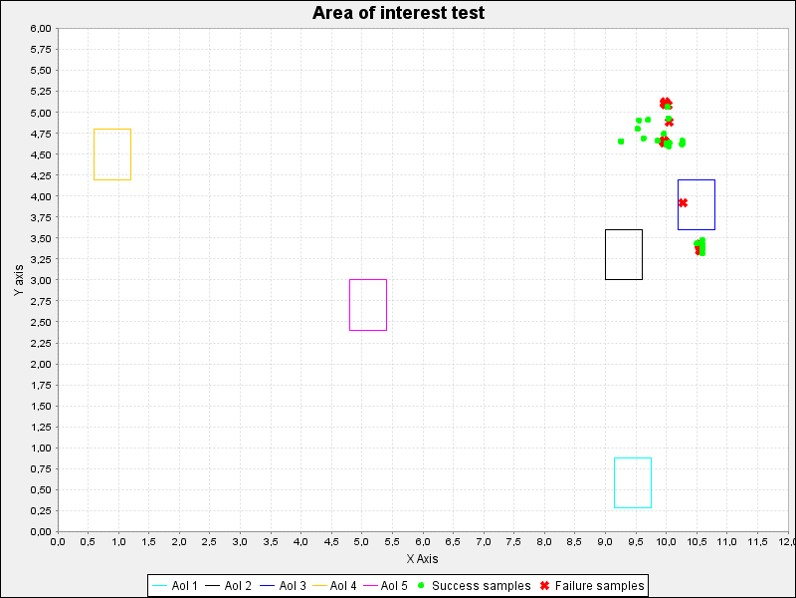
\includegraphics[width=0.6\textwidth]{images/eval_evaal_aoi}
\captionof{figure}{Recognition rate of CapFloor on selected areas of interest}
\label{fig:eval_evaal_aoi}
\end{minipage}

\begin{table}[htbp]
  \centering
  \caption{Best case scores of CapFloor @ EvAAL 2011}
    \begin{tabular}{rrr}
    \toprule
          & \multicolumn{2}{c}{Availability} \\
    \midrule
          & Run 1 & Run 2 \\
    Number of wrong samples & 210   & 258 \\
    Number of total received samples & 328   & 437 \\
    T     & 0.3597561 & 0.40961098 \\
    Accuracy Score & 3.59756098 & 4.09610984 \\
        \midrule
          & \multicolumn{2}{c}{Accuracy} \\
    Available samples & 358   & 437 \\
    Expected samples & 452   & 452 \\
    Availability & 0.7920354 & 0.96681416 \\
    Availability score & 7.92035398 & 9.66814159 \\
    \bottomrule
    \end{tabular}%
  \label{tab:evalres_capfloor}%
\end{table}%

\section{Smart Bed sleep phase recognition results}
\begin{minipage}{\linewidth}
\centering
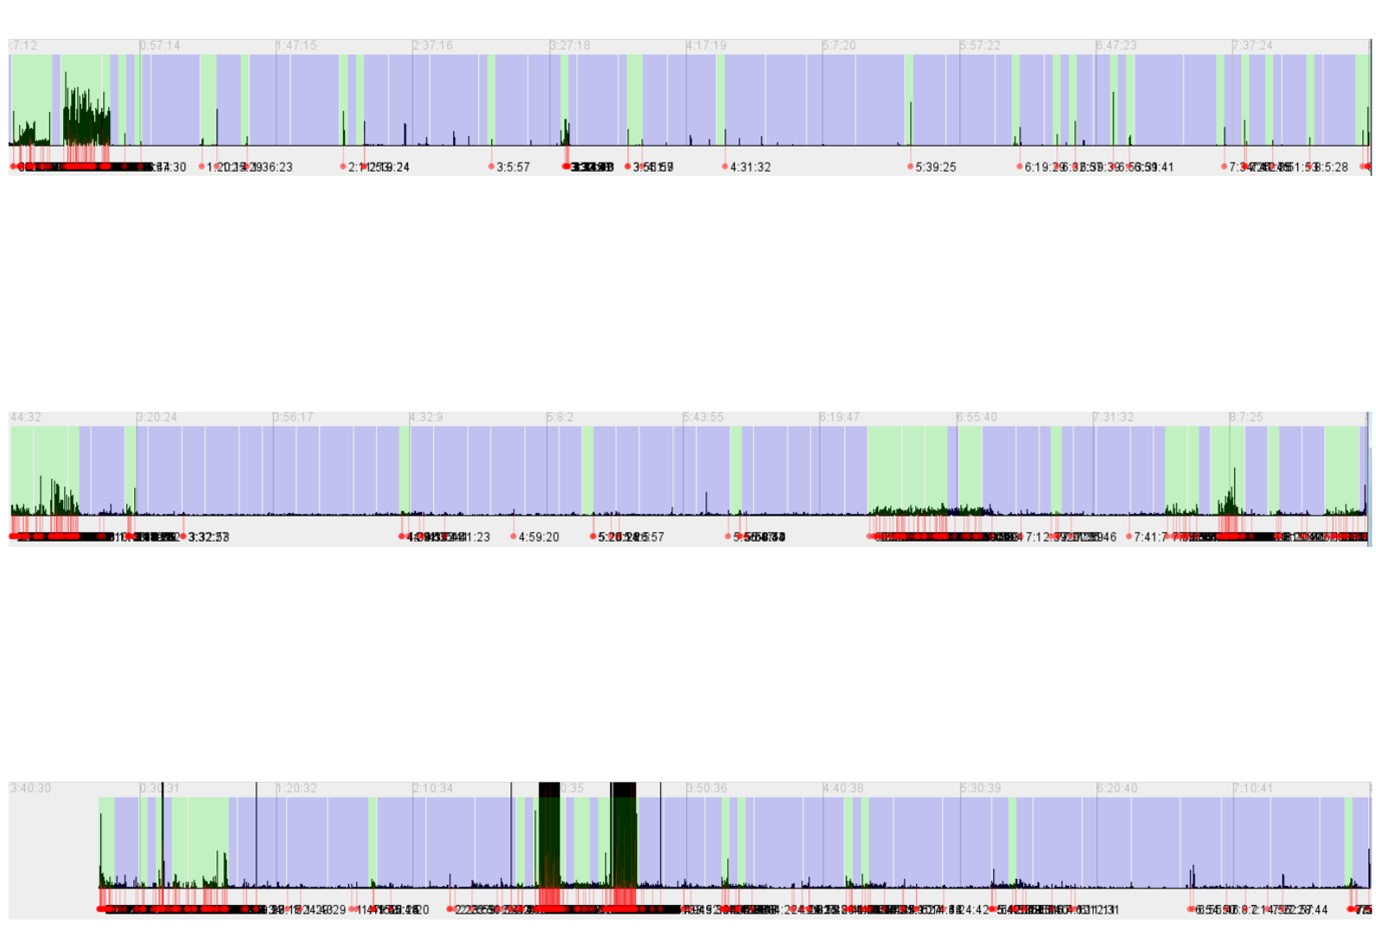
\includegraphics[width=1.0\textwidth]{images/eval_sleep_phase}
\captionof{figure}{Recognition of sleep phases over three nights}
\label{fig:eval_sleep_phase}
\end{minipage}





\chapter{Publications}
The thesis is partially based on the following publications:

\begin{description}
\item[2013]{\bf OpenCapSense: A Rapid Prototyping Toolkit for Pervasive Interaction Using Capacitive Sensing} (Tobias Grosse-Puppendahl, Yannick Berghoefer, Andreas Braun, Raphael Wimmer, Arjan Kuijper), {\em In IEEE International Conference on Pervasive Computing and Communications (PerCom)}, volume 18, pp. 22, 2013.
\item[2012]{\bf V2me: Evaluating the first steps in mobile friendship coaching} (Salla Muuraiskangas, Anja K Leist, Andreas Braun, Kerstin Klauß, Peter H M P Roelofsma, Reiner Wichert, Peter Klein, Dieter Ferring), {\em In Journal of Ambient Intelligence and Smart Environments}, IOS Press, volume 4, pp. 517-534, 2012.
\item[2011]{\bf User requirements in ICT-based social media use: Acceptance of a virtual coach} (Anja Leist, Dieter Ferring, Kerstin Klauss, Peter Klein, Andreas Braun, Reiner Wichert), {\em In }, 2011.
\item[2014]{\bf V2me - Virtual Coaching for Seniors} (Andreas Braun, Silvana Cieslik, René Zmugg, Reiner Wichert, Peter Klein, Sven Havemann), {\em In Wohnen – Pflege – Teilhabe - Besser leben durch Technik. 7. Deutscher AAL-Kongress}, VDE Verlag, 2014.
\item[2013]{\bf User requirements for navigation assistance in public transit for elderly people} (Stefanie Müller, Felix Kamieth, Andreas Braun, Tim Dutz, Peter Klein), {\em In Proceedings of the 6th International Conference on PErvasive Technologies Related to Assistive Environments}, pp. 55, 2013.
\item[2013] {\bf Swiss-cheese extended: an object recognition method for ubiquitous interfaces based on capacitive proximity sensing} (Tobias Grosse-Puppendahl, Andreas Braun, Felix Kamieth, Arjan Kuijper), {\em In Proceedings of the 2013 ACM annual conference on Human factors in computing systems}, pp. 1401-1410, 2013.
\item[2013]{\bf Context-based bounding volume morphing in pointing gesture applications} (Andreas Braun, Arthur Fischer, Alexander Marinc, Carsten Stocklöw, Martin Majewski), {\em In HCII'13 Proceedings of the 15th international conference on Human-computer interaction}, Springer Berlin Heidelberg, pp. 147-156, 2013.
\item[2013]{\bf Capacitive sensor-based hand gesture recognition in ambient intelligence scenarios} (Andreas Braun, Tim Dutz, Felix Kamieth), {\em In Proceedings of the 6th International Conference on PErvasive Technologies Related to Assistive Environments}, pp. 5, 2013.
\item[2013]{\bf Marker-Free Indoor Localization and Tracking of Multiple Users in Smart Environments Using a Camera-Based Approach} (Andreas Braun, Tim Dutz, Michael Alekseew, Philipp Schillinger, Alexander Marinc), {\em In Distributed, Ambient and Pervasive Interactions}, 2013.
\item[2012]{\bf Honeyfish - a high resolution gesture recognition system based on capacitive proximity sensing} (Tobias Grosse-Puppendahl, Andreas Braun), {\em In Embedded World Conference 2012}, Haar: WEKA Fachmedien, 2012 (Design \& Elektronik), pp. 10pp, 2012.
\item[2012]{\bf Context recognition using capacitive sensor arrays in beds} (Andreas Braun, Henning Heggen), {\em In Technik für ein selbstbestimmtes Leben - 5. Deutscher AAL-Kongress}, VDE VERLAG GmbH, 2012.
\item[2012]{\bf Visual Support System for Selecting Reactive Elements in Intelligent Environments} (Martin Majewski, Andreas Braun, Alexander Marinc, Arjan Kuijper), {\em In International Conference on Cyberworlds}, pp. 251-255, 2012.
\item[2012] {\bf CapFloor – A Flexible Capacitive Indoor Localization System} (Andreas Braun, Henning Heggen, Reiner Wichert), {\em In Evaluating AAL Systems Through Competitive Benchmarking. Indoor Localization and Tracking (Stefano Chessa, Stefan Knauth, eds.)}, Communications in Computer and Information Science, pp. 26-35, 2012.
\item[2011] {\bf Empowering and integrating senior citizens with virtual coaching} (Andreas Braun, Peter H. M. P. Roelofsma, Dieter Ferring, Milla Immonen), {\em In Ambient Intelligence (David V. Keyson, Mary Lou Maher, Norbert Streitz, Adrian Cheok, Juan Carlos Augusto, Reiner Wichert, Gwenn Englebienne, Hamid Aghajan, Ben J. A. Kröse, eds.)}, Springer Berlin Heidelberg, volume 7040, pp. 369-370, 2011.
\item[2011] {\bf Interactive personalization of ambient assisted living environments} (Alexander Marinc, Carsten Stocklöw, Andreas Braun, Carsten Limberger, Cristian Hofmann, Arjan Kuijper), {\em In Proceeding HI'11 Proceedings of the 2011 international conference on Human interface and the management of information}, volume Part I, pp. 567-576, 2011.
\item[2011] {\bf Passive identification and control of arbitrary devices in smart environments} (Andreas Braun, Felix Kamieth), {\em In HCII'11 Proceedings of the 14th international conference on Human-computer interaction: towards mobile and intelligent interaction environments (Julie A. Jacko, ed.)}, Springer-Verlag, pp. 147-154, 2011.
\item[2011] {\bf Adaptive implicit interaction for healthy nutrition and food intake supervision} (Felix Kamieth, Andreas Braun, Christian Schlehuber), {\em In HCII'11 Proceedings of the 14th international conference on Human-computer interaction: towards mobile and intelligent interaction environments}, Springer-Verlag, pp. 205-212, 2011.
\item[2011]{\bf Classification of User Postures with Capacitive Proximity Sensors in AAL-Environments} (Tobias Grosse-Puppendahl, Alexander Marinc, Andreas Braun), {\em In Ambient Intelligence (David V Keyson, Mary Lou Maher, Norbert Streitz, Adrian Cheok, Juan Carlos Augusto, Reiner Wichert, Gwenn Englebienne, Hamid Aghajan, Ben J A Kröse, eds.)}, Springer, volume 7040, pp. 314-323, 2011.
\item[2011] {\bf Designing a multi-purpose capacitive proximity sensing input device} (Andreas Braun, Pascal Hamisu), {\em In Proceedings of the 4th International Conference on PErvasive Technologies Related to Assistive Environments PETRA 11}, ACM Press, 2011.
\item[2010]{\bf Analyse des Schlafverhaltens durch kapazitive Sensorarrays zur Ermittlung der Wirbelsäulenbelastung} (Pascal Hamisu, Andreas Braun), {\em In 3. Deutscher AAL Kongress}, VDE VERLAG GmbH, pp. 3-6, 2010.
\item[2009] {\bf Using the human body field as a medium for natural interaction} (Andreas Braun, Pascal Hamisu), {\em In Proceedings of the 2nd International Conference on PErvsive Technologies Related to Assistive Environments - PETRA '09}, ACM Press, pp. 1-7, 2009.
\item[2012] {\bf Synergieeffekte aus der Kombination verschiedener AAL Lösungen} (Kerstin Klauß, Stefanie Müller, Andreas Braun, Tim Dutz, Felix Kamieth, Peter Klein), {\em In Mensch \& Computer 2012--Workshopband: interaktiv informiert--allgegenwärtig und allumfassend!? (H. Reiterer, O. Deussen, eds.)}, Oldenbourg Verlag, pp. 61-67, 2012.
\item[2013]{\bf Building Up Virtual Environments Using Gestures} (Alexander Marinc, Carsten Stocklöw, Andreas Braun), {\em In Chapter in Universal Access in Human-Computer Interaction. Applications and Services for Quality of Life}, Springer Berlin Heidelberg, pp. 70-78, 2013.
\item[2013]{\bf Providing Visual Support for Selecting Reactive Elements in Intelligent Environments} (Martin Majewski, Andreas Braun, Alexander Marinc, Arjan Kuijper), {\em In Chapter in Transactions on Computational Science XVIII}, Springer, pp. 248-263, 2013.
\item[2013]{\bf Unobtrusive Recognition of Working Situations} (Tobias Grosse-Puppendahl, Sebastian Benchea, Felix Kamieth, Andreas Braun, Christian Schuster), {\em In Chapter in Distributed, Ambient, and Pervasive Interactions}, Springer Berlin Heidelberg, pp. 115-121, 2013.
\item[2013]{\bf AmbiTrack-Marker-free Indoor Localization and Tracking of Multiple Users in Smart Environments with a Camera-based Approach} (Andreas Braun, Tim Dutz), {\em In Chapter in Evaluating AAL Systems Through Competitive Benchmarking}, Springer Berlin Heidelberg, pp. 83-93, 2013.
\item[2012]{\bf Dynamic User Representation in Video Phone Applications} (Andreas Braun, Reiner Wichert), {\em In Chapter in Constructing Ambient Intelligence}, Springer Berlin Heidelberg, pp. 184-188, 2012.
\end{description}

\newpage


\chapter{Supervising Activities}

The following list summarizes the student bachelor, diploma and master thesis supervised by the author. The results of these works were partially used as an input into the thesis.

\section{Diploma and Master Thesis}

\begin{enumerate}
\item Große-Puppendahl, Tobias - Multi-hand Interaction Using Custom Capacitive Proximity Sensors - MSc TU Darmstadt 2012 
\item Berghöfer, Yannick - Human-Machine-Interfaces in Automotive Environments using Capacitive Proximity Sensors - MSc TU Darmstadt 2013
\item Krepp, Stefan - Unobtrusive Surface Touch Recognition using Acoustic Tracking - MSc TU Darmstadt 2014
\item Frank, Sebastian - Vehicle-Integrated System for Person Health Management - MSc Hochschule Rhein-Main 2014
\end{enumerate}

\section{Bachelor Thesis}

\begin{enumerate}
\item Fischer, Arthur - Unterstützung von zielbasierter Interaktion durch gestenerkennende Zeigegeräte - BSc TU Darmstadt 2012
\item Majewski, Martin - Visual-aided Selection of Reactive Elements in Intelligent Environments - BSc TU Darmstadt 2012
\item Neumann, Stephan - Automotive interfaces using an interactive armrest - BSc TU Darmstadt 2014
\item Zander-Walz, Sebastian - Curved large-area surfaces for gestural interaction - BSc TU Darmstadt 2014
\end{enumerate}

\chapter{Curriculum Vitae }

\begin{cv}{}
  \begin{cvlist}{\textbf{Personal Data}}
 % \vspace{0.3cm}
  \item[Name] Andreas Braun
  \item[Birth date \& place] 04.10.1982 Aschaffenburg, Germany
	\item[Nationality] German
\end{cvlist}

\vspace{1cm}

\begin{cvlist}{\textbf{Education}} 
  %\vspace{0.3cm}
\item[2008 -- 2010] Master of Science in Computational Engineering at Technical University of Darmstadt, Germany
\item[2004 -- 2008] Bachelor of Science in Computational Engineering at Technical University of Darmstadt, Germany
\item[2002 -- 2004] Study of Physics at Julius-Maximilians Universität in Würzburg, Germany
\end{cvlist}

\vspace{1cm}

\begin{cvlist}{\textbf{Work Experience}}
%  \vspace{0.3cm}
\item[2010 --] Researcher, Competence Center Interactive Multimedia Appliances, Fraunhofer Institute for Computer Graphics Research, Darmstadt, Germany, Focus: HCI applications in smart environments
\item[2008 -- 2009] Student Assistant, Competence Center Interactive Multimedia Appliances, Fraunhofer Institute for Computer Graphics Research, Darmstadt, Germany, Focus: Sensor applications and interactive systems
\end{cvlist}

\date{}
\end{cv}






 

\end{appendix}




